%%%%%%%%%%%%%%%%%%%%%%%%%%%%%%%%%%%%%%%%%
% NIWeek 2014 Poster by T. Reveyrand
% www.microwave.fr
% http://www.microwave.fr/LaTeX.html
% ---------------------------------------
% 
% Original template created by:
% Brian Amberg (baposter@brian-amberg.de)
%
% This template has been downloaded from:
% http://www.LaTeXTemplates.com
%
% License:
% CC BY-NC-SA 3.0 (http://creativecommons.org/licenses/by-nc-sa/3.0/)
%
%%%%%%%%%%%%%%%%%%%%%%%%%%%%%%%%%%%%%%%%%

%----------------------------------------------------------------------------------------
%	PACKAGES AND OTHER DOCUMENT CONFIGURATIONS
%----------------------------------------------------------------------------------------
\documentclass[a0paper,portrait]{baposter}
\usepackage{amsmath,amsfonts,amssymb,amsthm} 
\usepackage[font=small,labelfont=bf]{caption} % Required for specifying captions to tables and figures
\usepackage{booktabs} % Horizontal rules in tables
\usepackage{multirow}
\usepackage{color, colortbl}
\usepackage{relsize} % Used for making text smaller in some places
\usepackage{siunitx}
\usepackage{physics}
\usepackage{fontspec} % only works with LuaTeX
\usepackage{eqparbox}
\usepackage{graphicx}
\usepackage{textcomp}
\usepackage[utf8]{inputenc}
\usepackage{xargs}
\usepackage{subcaption}
\captionsetup[subfigure]{labelformat=parens}

\newcommandx{\myfig}[5][3=50pt,4=0.7,5=0.27]{
\begin{minipage}{\textwidth}
\centering
\raisebox{-#3}{\includegraphics[width=#4\textwidth]{#1}}
\parbox[c]{#5\textwidth}{\captionof{figure}{#2}}
\end{minipage}
}

\newcommandx{\myfigb}[5][3=0pt,4=0.5,5=1]{
\begin{minipage}{#4\textwidth}
\centering
\includegraphics[width=#5\textwidth]{#1}
\captionof{figure}{#2}
\end{minipage}
}
%----------------------------------------------------------------------------------------


%----------------------------------------------------------------------------------------
%	DEFAULT POSTER CONFIGURATIONS
%----------------------------------------------------------------------------------------
\definecolor{mainblue}{RGB}{51,133,255}
\definecolor{bblue}{RGB}{220, 235, 250}
\definecolor{brose}{RGB}{245, 215, 215}

\def \postercodepx{0.875\paperwidth}
\def \postercodepy{0.975\paperheight}
\def \posterlinewidth{5pt}
\def \posterlineheight{0.89\paperheight}
\def \posternrcolumns{4}
\def \rightlogowidth{0.24\textwidth}
\def \leftlogowidth{0.18\textwidth}
\graphicspath{{figures/}} % Directory in which figures are stored

\setmainfont{Arial}  % Command related to fontspec package. Comment this line and comment the next if you are not using the XeTeX or the LuaTeX engine
%\renewcommand{\familydefault}{\sfdefault} 
%----------------------------------------------------------------------------------------


%----------------------------------------------------------------------------------------
%	HEADER INFO
%----------------------------------------------------------------------------------------
\def \rightlogo{cnpem_logo.png}
\def \leftlogo{ipac22_logo.png}
\def \postercode{THPOPT056}
\def \postertitle{Emittance Exchange at SIRIUS Booster for Storage Ring Injection Improvement}
\def \posterauthors{J. V. Quentino, \underline{M. B. Alves}, F. H. de Sá}
\def \posteremail{murilo.alves@lnls.br}
%----------------------------------------------------------------------------------------


\begin{document}

\begin{poster}{
grid=false,
columns=\posternrcolumns,
borderColor=mainblue, % Border color of content boxes
headerFontColor=black, % Text color for the header text in the content boxes
headerColorOne=white, % Background color for the header in the content boxes (left side)
headerColorTwo=white, % Background color for the header in the content boxes (right side)
boxColorOne=white, % Background color for the content in the content boxes
headerfont=\large\bf, % Font modifiers for the text in the content box headers
headerborder=open, % Change to closed for a line under the content box headers
textborder=rectangle,
background=None,
boxshade=plain
}
{
\includegraphics[width=\rightlogowidth]{\rightlogo}
}
{ 
\textcolor{mainblue}{\LARGE{\bf{\postertitle}}} 
\vspace{0.2cm}
} 
{
\large{\posterauthors} \\
\footnotesize{\posteremail} \\
\medskip
\textcolor{mainblue}{\textit{\normalsize{Brazilian Synchrotron Light Laboratory, LNLS, Brazil}}}  
} 
{
\includegraphics[width=\leftlogowidth]{\leftlogo}
}

\node[draw=none,fill=none] at (\postercodepx,\postercodepy){\postercode};
\draw[draw=mainblue,line width=\posterlinewidth] (-10,\posterlineheight)  --  (\paperwidth, \posterlineheight);

%----------------------------------------------------------------------------------------
%	POSTER BOXES
%----------------------------------------------------------------------------------------


\headerbox{\textit{Abstract}}{
name=abstract,
column=0,
span=\posternrcolumns,
headerfont=\large\bf,
borderColor=white}{
   SIRIUS is the new 4\textsuperscript{th} generation storage ring based synchrotron light source built and operated by the Brazilian Synchrotron Light Laboratory (LNLS) at the Brazilian Center for Research in Energy and Materials (CNPEM). %\
   Currently, the efficiency of the horizontal off-axis injection system of the storage ring is still not suitable for top-up operation due to a smaller than expected horizontal dynamic aperture. In this work, we report the simulations and experimental results of transverse emittance exchange (TEE) performed at SIRIUS booster by crossing a coupling difference resonance during energy ramp, with the goal of decreasing the injected horizontal beam size and improve the off-axis injection efficiency.
}

\headerbox{\MakeUppercase{Crossing speed and TEE quality}}{
name=step,
column=0,
span=2,
below=abstract}{
The TEE adiabaticity is described by the following scaling parameter:   
\begin{equation}
S = \frac{\dot{\Delta}}{|C|^2}
\end{equation}
while the exchange quality is computed by:
\begin{equation}
    R = 1 - \frac{\epsilon_x - \epsilon_{y0}}{\epsilon_{x0} - \epsilon_{y0}},
    \label{eq:r_def}
\end{equation}
\myfig
{THPOPT056_f1.pdf}
{Emittance exchange quality as function of coupling coefficient $|C|$ and the time to cross the difference resonance $t_c$. The dashed lines indicate curves with constant $S$ and emittance exchange quality higher than $\SI{80}{\%}$.
% The results were obtained by tracking the beam envelope and updating, turn-by-turn, the one-turn map and diffusion matrices to perform the TEE process.
}
[60 pt][0.5][0.47]
}

\headerbox{\MakeUppercase{SIMULATION OF INJECTION WITH TEE}}{
name=inj,
column=0,
span=2,
below=auto}{
    \begin{center}
        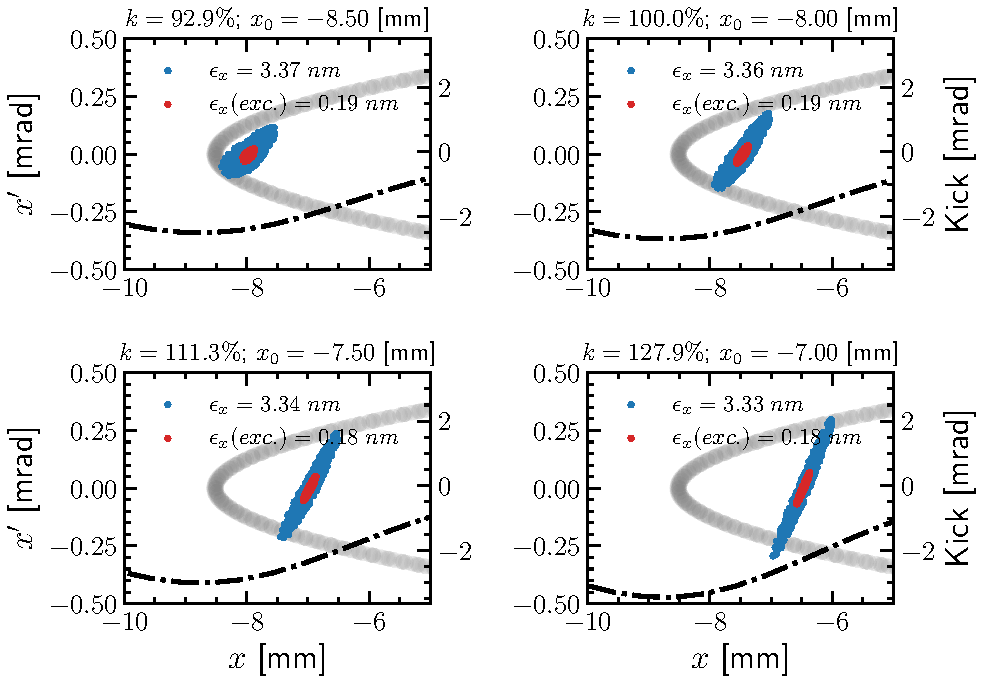
\includegraphics[width=0.85\linewidth]{NLK_effect.pdf}
    \captionof{figure}{Phase-space diagrams of the bunch after the NLK for different initial horizontal positions $x_0$ at the NLK entrance. The dash-dotted lines represent the NLK pulse in units of angular kick. At each initial position, the NLK kick was optimized to deliver the bunch with $\expval{x'} \approx 0$, the parameter $k$ express the pulse intensity relative to the pulse used to align the bunch with $x_0 = - \SI{8.00}{\milli \meter}$.
    }
    \end{center}
}

\headerbox{\MakeUppercase{Booster coupling measurement}}{
name=inj,
column=0,
span=2,
below=auto,
above=bottom}{
\begin{minipage}{0.38\textwidth}
\captionof{table}{SIRIUS booster nominal parameters at extraction energy.}
\resizebox{\textwidth}{!}{
  \begin{tabular}{lc}
      \toprule
      Energy ramp & $\SI{150}{\mega \electronvolt}$ to $\SI{3}{\giga\electronvolt}$ \\ 
      Tunes & $19.204, \;7.314$ \\ 
      Energy spread &  $\SI{0.087}{\%}$ \\ 
      Natural emittance & $\SI{3.5}{\nano \meter\radian}$ \\
      Damping times & $\SI{11.3}{\milli\second}, \SI{13.7}{\milli\second}$ \\
      Ramp up duration & $\approx \SI{300}{\milli\second}$ \\
      Repetition rate & $\SI{2}{\hertz}$\\
    %   \midrule
      \bottomrule
  \end{tabular}}
  
  \vspace{0.3cm}
\begin{center}
Measured \textbf{coupling}:    
\end{center}
\[|C| = \SI{0.6 \pm 0.3}{\%}\]
%   By the closest tune approach method, we find a coupling coefficient modulus of $|C|=0.61 \pm 0.27~\%$.
\end{minipage}
 \hfill
\begin{minipage}[c]{0.59\textwidth}
    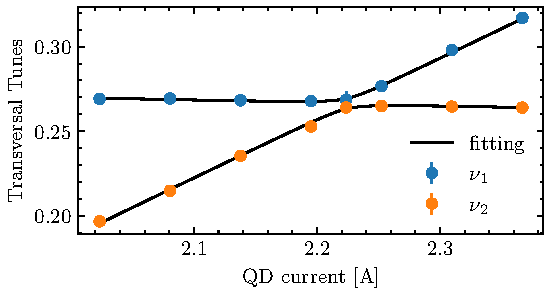
\includegraphics[width=\textwidth]{THPOPT056_f3.pdf}
  \captionof{figure}{Closest tune approach method for measurement of natural betatron coupling close to extraction energy.}
\end{minipage}

}

\headerbox{\MakeUppercase{Emittance exchange implementation}}{
name=traj,
column=2,
span=2,
below=abstract}{ 

\begin{center}
    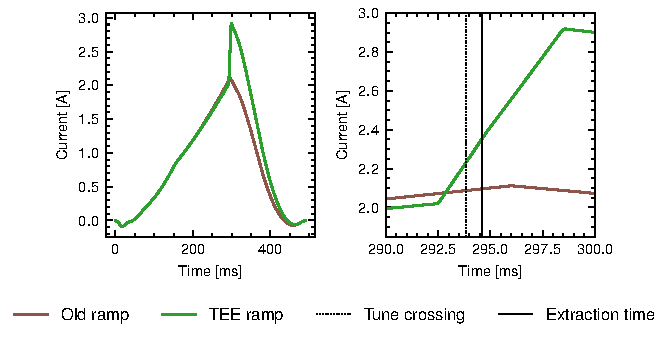
\includegraphics[width=0.8\textwidth]{THPOPT056_f4.pdf}
    \captionof{figure}{Modification made in QD quadrupoles current ramp to implement the TEE. On the left, the full ramp is shown and a zoom with the details around the extraction point is on the right plot.}
\end{center}

}


\headerbox{\MakeUppercase{Evaluating the exchange quality}}{
name=orb,
column=2,
span=2,
below=traj}{

\begin{center}
   \myfig
{THPOPT056_f5a.pdf}
{Beam sizes during emittance exchange.}
[70pt][0.65][0.3]
\end{center}

% I had to include the above figure manually because was needed to crop the image.
\begin{minipage}{0.55\textwidth}
The emittances can be estimated using the following equation with nominal values for energy spread and optical functions:
\[\epsilon_{x, y} = \frac{\sigma_{x, y}^2 - (\sigma_\delta \eta_{x,y})^2}{\beta_{x, y}} \]
\end{minipage}
\hfill
\begin{minipage}{0.4\textwidth}
% \vspace{-2.1cm}
\captionof{table}{Nominal optical functions at the YAG screen in the booster-to-storage ring transport line.}
\resizebox{\textwidth}{!}{
  \begin{tabular}{lc}
      \toprule
      $\beta_x, \; \beta_y$ & $\SI{17.11}{m}, \; \SI{6.60}{m}$ \\ 
      $\eta_x, \; \eta_y$ & $\SI{-13}{cm}, \; \SI{0}{cm}$ \\ 
      \bottomrule
  \end{tabular}}
\end{minipage}
\vspace{0.4cm}
\begin{minipage}{1\textwidth}
\centering
\raisebox{-50pt}{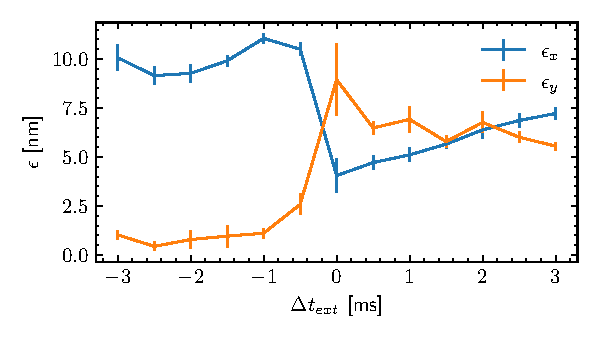
\includegraphics[trim={0.4cm 0.4cm 0 0}, clip, width=0.67\textwidth]{THPOPT056_f5b.pdf}}
\parbox[c]{0.3\textwidth}{\captionof{figure}{Estimate of emittances behavior using nominal optical functions.}}
% \captionof{figure}{Estimate of emittances behavior during the exchange using nominal optical functions.}
\end{minipage}

% \vspace{0.5cm}
Based on this estimation, the \textbf{exchange quality} at the extraction energy is:
\[ R = \SI{70 \pm 10}{\%}\]

}

\headerbox{\MakeUppercase{Injection efficiency}}{
name=rf,
column=2,
span=2,
below=orb,
above=bottom}{ 
\begin{center}
\begin{minipage}{0.65\textwidth}
\captionof{table}{Injection efficiency comparison}
\resizebox{\textwidth}{!}{
  \centering
  \begin{tabular}{lcc}
      \toprule
      & Before TEE & After TEE \\
      \midrule
      Optimized Inj. System & $\SI{86}{\%}$ & $\SI{96}{\%}$ \\ 
      User shifts & $\SI{75}{\%}$ & $\SI{82}{\%}$ \\ 
      \bottomrule
  \end{tabular}}
\end{minipage}
\end{center}
\vspace{0.1cm}

% \begin{minipage}{0.44\textwidth}
\small{In addition, we also observed a lower correlation between injection efficiency and pulsed magnets temperatures after the TEE implementation.}
% \end{minipage}

}

% \headerbox{\MakeUppercase{References}}{
% name=rf,
% column=2,
% span=2,
% below=rf,
% above=bottom}{ }
\end{poster}

\end{document}